% LNCS paper: Unsupervised anomaly detection in multivariate sensor time series.
% Compile on Overleaf with the Springer LNCS template (needs llncs.cls and
% splncs04.bst from that template). Upload this file, references.bib and the
% figures/ folder into the template project.
\documentclass[runningheads]{llncs}

\usepackage[T1]{fontenc}
\usepackage{graphicx}
\usepackage{amsmath,amssymb}
\usepackage{booktabs}
\usepackage{tikz}
\usetikzlibrary{arrows.meta,positioning}
\usepackage{hyperref}
\usepackage{color}
\renewcommand\UrlFont{\color{blue}\rmfamily}

% Shows the figure if present, otherwise a placeholder box so the paper always
% compiles before the PNGs are uploaded.
\newcommand{\plot}[2]{%
  \IfFileExists{#1}{\includegraphics[#2]{#1}}%
  {\fbox{\parbox[c][4cm][c]{0.9\linewidth}{\centering\small\texttt{#1}\\(upload figure)}}}}

\begin{document}

\title{Unsupervised Anomaly Detection in Multivariate Industrial Sensor Time Series with a Dilated Convolutional Autoencoder and Per-Sensor Mahalanobis Scoring}
\titlerunning{Dilated CNN Autoencoder with Mahalanobis Scoring}

\author{Bhuvana Shikaripura Dasharatha \and Purna Chandra Nandigana}
\authorrunning{B. Shikaripura Dasharatha and P. C. Nandigana}

\institute{RPTU Kaiserslautern-Landau, Kaiserslautern, Germany}
% \email{...}  % add author e-mail addresses if required

\maketitle

\begin{abstract}
We detect anomalous timesteps in 18-sensor recordings of an industrial batch-distillation process. The training runs carry no labels, so we treat the task as novelty detection. A dilated, residual 1D convolutional autoencoder learns to reconstruct normal sensor windows. Its per-sensor reconstruction error is scored by Mahalanobis distance under a Ledoit--Wolf covariance estimate, and a threshold is chosen on a small labelled validation set. Replacing flat mean-squared error with per-sensor Mahalanobis scoring was the largest single improvement, raising validation F1 from 0.48 to about 0.60 and ROC-AUC from 0.65 to 0.76; the external competition portal scored the submission at F1 = 0.63. Fusing the autoencoder with Isolation Forest or Local Outlier Factor detectors, with the fusion weight chosen by run-grouped cross-validation, did not improve on the autoencoder alone. A leave-one-run-out analysis further shows that the standard validation protocol is optimistic: fitting the Mahalanobis model on normal windows from the same runs being scored inflates ROC-AUC by 0.07 and F1 by 0.06. We report these negative results alongside the positive ones.

\keywords{Anomaly detection \and Multivariate time series \and Convolutional autoencoder \and Mahalanobis distance \and Industrial sensors}
\end{abstract}

%======================================================================
\section{Introduction}
%======================================================================

Industrial processes are monitored by many sensors, and faults usually show up as departures from the joint behaviour of those sensors rather than as a single out-of-range reading. Detecting such departures automatically is a standard problem in multivariate time-series anomaly detection~\cite{malhotra2016lstm,hundman2018detecting,audibert2020usad}.

Our data come from an industrial batch-distillation process with 18 sensors (temperatures, pressures, flows). The setting has one constraint that shapes every design decision: the 28 training runs are unlabelled. Only 10 validation runs carry per-timestep labels, and 53 test runs are scored by an external competition portal. A supervised classifier is therefore not an option. We instead learn a model of normal behaviour and flag timesteps that deviate from it.

The contributions of this paper are:
\begin{enumerate}
  \item A dilated residual convolutional autoencoder (TCN-style~\cite{bai2018empirical,oord2016wavenet}) whose receptive field covers the slow drifts that characterise the anomalies in this data.
  \item Per-sensor Mahalanobis scoring of reconstruction error, which prevents a genuine deviation on one sensor from being averaged away by ordinary noise on the others. This change alone raised validation F1 from 0.48 to about 0.60.
  \item A controlled fusion study showing that neither Isolation Forest~\cite{liu2008isolation} nor Local Outlier Factor~\cite{breunig2000lof} adds to the autoencoder when the fusion weight is chosen without leakage.
  \item An analysis of the evaluation protocol itself. Leave-one-run-out calibration shows the usual validation estimate is optimistic, and arithmetic on the portal result shows it is inconsistent with point-wise F1 at the validation anomaly rate.
\end{enumerate}

%======================================================================
\section{Data and Problem Setting}
%======================================================================

Each run is a multivariate time series of 18 sensor channels. Table~\ref{tab:data} summarises the splits. The validation labels mark 19{,}086 of 79{,}688 timesteps as anomalous, a prevalence of 0.2395. Anomaly prevalence varies strongly between validation runs, from 0.8\% to 81\% of timesteps. The test labels are not available locally, and the portal's metric and the test prevalence are not documented.

\begin{table}[t]
\centering
\caption{Data splits.}\label{tab:data}
\begin{tabular}{lrl}
\toprule
Split & Runs & Labels \\
\midrule
Train & 28 & none \\
Validation & 10 & per-timestep 0/1 (prevalence 0.2395) \\
Test & 53 & none locally; scored by external portal \\
\bottomrule
\end{tabular}
\end{table}

The task is to output a binary prediction for every test timestep. We fit a standard scaler on the training runs only and apply it to all splits.

%======================================================================
\section{Method}
%======================================================================

Figure~\ref{fig:pipeline} shows the pipeline. Labels are used for two decisions only: selecting the training checkpoint and selecting the decision threshold.

\begin{figure}[t]
\centering
\resizebox{0.85\linewidth}{!}{%
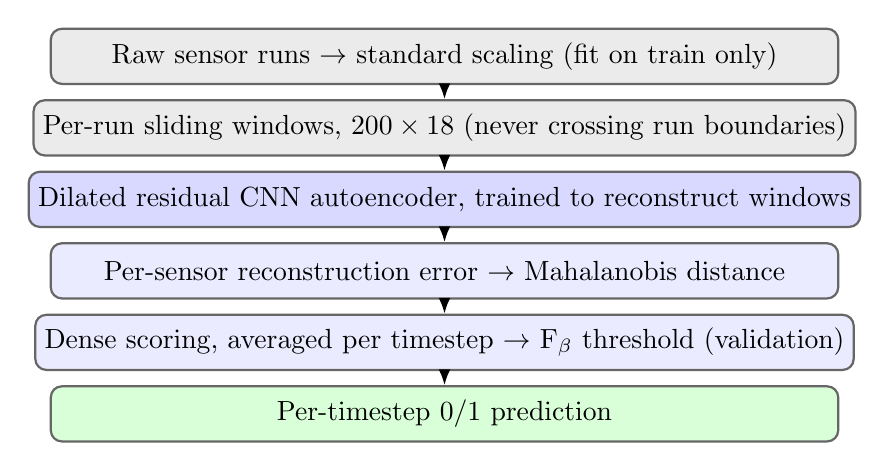
\begin{tikzpicture}[
  node distance=0.18cm,
  box/.style={rectangle, rounded corners, draw=black!60, thick, minimum width=10cm, minimum height=0.7cm, align=center},
  arr/.style={-{Latex[length=2mm]}, thick}]
\node[box, fill=black!8] (n1) {Raw sensor runs $\rightarrow$ standard scaling (fit on train only)};
\node[box, fill=black!8, below=of n1] (n2) {Per-run sliding windows, $200 \times 18$ (never crossing run boundaries)};
\node[box, fill=blue!15, below=of n2] (n3) {Dilated residual CNN autoencoder, trained to reconstruct windows};
\node[box, fill=blue!8, below=of n3] (n4) {Per-sensor reconstruction error $\rightarrow$ Mahalanobis distance};
\node[box, fill=blue!8, below=of n4] (n5) {Dense scoring, averaged per timestep $\rightarrow$ F$_\beta$ threshold (validation)};
\node[box, fill=green!15, below=of n5] (n6) {Per-timestep 0/1 prediction};
\foreach \i/\j in {1/2,2/3,3/4,4/5,5/6} \draw[arr] (n\i) -- (n\j);
\end{tikzpicture}}
\caption{Detection pipeline.}\label{fig:pipeline}
\end{figure}

\subsection{Windowing}

We cut each run into windows of $T = 200$ timesteps across all $D = 18$ sensors. Windows are built per run and never span two runs. Training windows use stride 10. Validation and test windows use stride 1, and each timestep's score is the mean of the scores of all windows that contain it, which gives exactly one score per timestep.

\subsection{Dilated Convolutional Autoencoder}

The encoder is a stack of four residual blocks with dilations 1, 2, 4 and 8. Each block contains two 1D convolutions (kernel size 3) with batch normalisation and ReLU, plus a residual connection (a $1\times1$ convolution when channel counts differ). Channel widths are 32, 32, 32 and 64. Max-pooling by a factor of 2 forms the bottleneck ($64 \times 100$). The decoder upsamples with a transposed convolution to $32 \times 200$, applies two residual blocks with dilations 4 and 2, and projects back to 18 channels with a final convolution.

The encoder's receptive field is 61 timesteps, compared with 3 for the single-layer convolution in our first version. The wider context matters because the anomalies in this process are mostly slow drifts rather than one-step spikes. The bottleneck prevents the network from learning the identity map, which would also reconstruct anomalies well.

The model is trained with mean-squared reconstruction loss, Adam (learning rate $10^{-3}$), batch size 64, for up to 50 epochs. Training loss decreases steadily with no plateau, and validation quality is not monotonic in the epoch count, so we evaluate every 5 epochs and keep the checkpoint with the best validation F$_\beta$.

\subsection{Per-Sensor Mahalanobis Scoring}

Averaging squared error over all sensors and timesteps produces a single number in which a large error on one precise sensor is diluted by ordinary noise on the other 17. We instead keep one error value per sensor: for window $w$, let $e_w \in \mathbb{R}^{18}$ be the mean squared reconstruction error of each sensor over the window. We fit a Gaussian model of normal error with mean $\mu$ and covariance $\Sigma$, estimating $\Sigma$ with Ledoit--Wolf shrinkage~\cite{ledoit2004well} for numerical stability, and score each window by
\begin{equation}
  s(w) = (e_w - \mu)^\top \Sigma^{-1} (e_w - \mu).
\end{equation}
In our pipeline, $\mu$ and $\Sigma$ are fitted on validation windows whose labels are all normal. Section~\ref{sec:protocol} examines the consequences of this choice.

As an example from the validation data, one window in which sensor FT703 rises to $z = +5.99$ while T701 stays flat produces $s(w) \approx 1058$, far above the threshold of about 43, and is correctly flagged. Under flat MSE the same deviation would be averaged across all 18 sensors.

\subsection{Threshold Selection}

The normal and anomalous score distributions overlap, and choosing the threshold that maximises F1 on validation flagged a large share of timesteps. We therefore sweep the precision--recall curve and pick the threshold that maximises F$_\beta$ with $\beta = 0.5$, which weights precision more heavily. We also report ROC-AUC, which measures ranking quality independent of the threshold.

%======================================================================
\section{Experiments}
%======================================================================

All numbers in this section are validation metrics unless a portal score is named explicitly. Random seeds are fixed at 42. Repeated runs of identical configurations still vary by about $\pm 0.02$ F1 (observed range 0.568--0.611) because of non-deterministic GPU training, so differences smaller than that are not evidence of improvement.

\subsection{Development History}

Table~\ref{tab:journey} lists the changes in the order they were made. The first row follows a rebuild of the codebase that fixed several correctness bugs, the most important of which was switching from window-level to per-timestep evaluation. Earlier, higher-looking numbers were computed at window level and are not comparable.

\begin{table}[t]
\centering
\caption{Validation results after each development step.}\label{tab:journey}
\begin{tabular}{lcc}
\toprule
Step & F1 & ROC-AUC \\
\midrule
Rebuilt pipeline, per-timestep evaluation & 0.41 & -- \\
+ Checkpoint selection & 0.46 & -- \\
+ Dilated residual architecture & 0.48 & 0.65 \\
+ Per-sensor Mahalanobis scoring + F$_{0.5}$ threshold & \textbf{0.58--0.60} & \textbf{0.76} \\
\midrule
Competition portal (test set) & \textbf{0.63} & -- \\
\bottomrule
\end{tabular}
\end{table}

The largest improvement came from changing how the score is computed, with no change to the network. The ROC-AUC increase from 0.65 to 0.76 shows that this was a real improvement in separating anomalies from normal data, not only a better threshold. The final model of record reaches validation F1 = 0.602 (precision 0.600, recall 0.605) and ROC-AUC 0.763. The portal scored its test predictions at F1 = 0.63.

\subsection{Fusion with Tabular Detectors}

We tested whether a detector built on different features could cover the autoencoder's blind spots. We first fused the autoencoder with an Isolation Forest~\cite{liu2008isolation} trained on per-window summary statistics, then with a Local Outlier Factor detector~\cite{breunig2000lof} trained on cross-sensor features (pairwise differences and rolling correlations). Scores were combined as a weighted sum. For LOF, the weight was chosen by 5-fold cross-validation grouped by run, so no run contributes to both weight selection and evaluation, and we report the out-of-fold F1.

\begin{table}[t]
\centering
\caption{Fusion study (validation). The fusion weight search was allowed to select the autoencoder alone.}\label{tab:fusion}
\begin{tabular}{lccc}
\toprule
Model & F1 & ROC-AUC & Selected LOF weight \\
\midrule
CNN autoencoder only & \textbf{0.59} & \textbf{0.77} & -- \\
LOF only & 0.46--0.48 & 0.67 & -- \\
CNN + LOF (out-of-fold) & 0.55 & 0.72 & 0.03 (raw) / 0.00 (standardised) \\
\bottomrule
\end{tabular}
\end{table}

Table~\ref{tab:fusion} shows the result. In 9 of 10 folds across the two LOF variants, the weight search chose the autoencoder alone. Even small LOF weights increased recall but reduced precision, lowering F1. The Isolation Forest fusion behaved the same way and always selected a CNN weight of 1.0. The tabular detectors rank anomalies less well than the autoencoder (ROC-AUC about 0.67 against 0.77), and mixing a weaker score into a stronger one degraded it. We therefore use the autoencoder alone.

\subsection{Failure Analysis}

Figure~\ref{fig:dist} shows that the score distributions of normal and anomalous timesteps overlap heavily near zero. This overlap limits achievable ROC-AUC, and no choice of threshold removes it. Per-sensor error analysis shows that most of the signal comes from flow and pressure sensors (FT703, T703, FT704, PDI702, FYI702).

\begin{figure}[t]
\centering
\plot{figures/score_distributions.png}{width=0.8\linewidth}
\caption{Distribution of anomaly scores for normal and anomalous validation timesteps.}\label{fig:dist}
\end{figure}

Per-run results vary widely (Fig.~\ref{fig:timelines}). Two validation runs score F1 = 0: in both, the score peaks coincide with the labelled anomalies but stay below the global threshold, because raw score magnitudes differ by about two orders of magnitude between runs.

\begin{figure}[t]
\centering
\plot{figures/val_score_timelines.png}{width=\linewidth}
\caption{Anomaly score over time for each validation run, with labelled anomalies and the global threshold.}\label{fig:timelines}
\end{figure}

\subsection{Follow-Up Experiments}

After the model of record was fixed, we tested three changes. All variants in each comparison share one trained network, so differences reflect the variant rather than training noise. Table~\ref{tab:followup} summarises them.

\begin{table}[t]
\centering
\caption{Follow-up experiments on one shared network (validation). ``Flagged'' is the fraction of timesteps predicted anomalous.}\label{tab:followup}
\begin{tabular}{lcccc}
\toprule
Variant & F1 & ROC-AUC & Val flagged & Test flagged \\
\midrule
Reference: val-normal fit, F$_{0.5}$ threshold & 0.583 & 0.769 & 0.244 & 0.617 \\
F1 threshold instead of F$_{0.5}$ & 0.607 & 0.769 & 0.360 & 0.842 \\
Per-run median/MAD score normalisation & 0.405 & 0.677 & 0.099 & 0.102 \\
Mahalanobis model fitted on train windows & 0.483 & 0.611 & 0.455 & 0.833 \\
\bottomrule
\end{tabular}
\end{table}

\paragraph{Threshold objective.} Choosing the threshold for F1 rather than F$_{0.5}$ raised validation F1 by 0.024, which is within the run-to-run variation. On the test set the same threshold flags 84\% of timesteps, so we did not adopt it.

\paragraph{Per-run normalisation.} Rescaling each run's scores by its median and median absolute deviation was intended to fix the two runs with F1 = 0. Instead it reduced ROC-AUC from 0.769 to 0.677. Because ROC-AUC is threshold-independent, the normalisation damaged the ranking itself, most likely by removing genuine differences between runs.

\paragraph{Fitting the normal model on training data.} Fitting $\mu$ and $\Sigma$ on all training windows instead of normal validation windows reduced ROC-AUC to 0.611. Training-window errors are much tighter than errors on held-out normal windows: per-sensor error variance is 0.000144 on training windows against 0.001727 on normal validation windows. This is expected, since the network was trained on those windows. The two fits also differ in contamination and in whether they share runs with the scored data, so this experiment does not isolate a single cause. A third fit on all validation windows, including anomalies (ROC-AUC 0.693), still beats the training-data fit, which suggests contamination alone does not explain the gap.

%======================================================================
\section{How Reliable Is the Evaluation?}\label{sec:protocol}
%======================================================================

\subsection{Same-Run Calibration Is Optimistic}

The Mahalanobis model in our pipeline is fitted on normal windows from the same validation runs it then scores. Test runs cannot provide such windows. To measure the effect, we re-scored each validation run with a model fitted only on the other nine runs (leave-one-run-out, Table~\ref{tab:loro}).

\begin{table}[t]
\centering
\caption{Effect of leave-one-run-out (LORO) calibration of the Mahalanobis model.}\label{tab:loro}
\begin{tabular}{lccccc}
\toprule
Calibration & ROC-AUC & F1 & Precision & Recall & Flagged \\
\midrule
Same runs (pipeline default) & 0.769 & 0.583 & 0.577 & 0.589 & 0.244 \\
Leave-one-run-out & 0.699 & 0.525 & 0.462 & 0.609 & 0.316 \\
\bottomrule
\end{tabular}
\end{table}

ROC-AUC falls by 0.070 and F1 by 0.058, and per-run ROC-AUC decreases in every one of the ten runs. The validation numbers in Table~\ref{tab:journey} should therefore be read as optimistic estimates. Compared against this leave-one-run-out baseline rather than the default, the training-data fit's ROC-AUC deficit shrinks from 0.158 to 0.088.

\subsection{What Does the Portal Measure?}

Our portal submission flags 62.2\% of test timesteps and scored 0.63. If the portal computed point-wise F1, a submission that flags a fraction $q$ of timesteps on a test set with anomaly prevalence $p$ and recall $r$ would score
\begin{equation}
  F_1 = \frac{2\,r\,p}{q + p}.
\end{equation}
With $q = 0.622$ and $p = 0.2395$ (the validation prevalence), even perfect recall gives at most $F_1 = 0.556$. Reaching 0.63 requires $p \geq 0.286$ at perfect recall, or $p \geq 0.44$ at the model's validation recall of 0.76. Either the test set has far more anomalies than the validation set, or the portal uses a different metric, such as point-adjusted or event-wise F1, which are known to reward flagging generously~\cite{kim2022towards}. The available documentation does not say which. Until that is known, choosing a threshold for the portal is guesswork.

%======================================================================
\section{Conclusion}
%======================================================================

A dilated residual autoencoder with per-sensor Mahalanobis scoring detects anomalies in unlabelled 18-sensor process data with validation F1 of about 0.60 and portal F1 of 0.63. The scoring change contributed more than any architecture change. Fusion with tabular detectors, per-run normalisation, and fitting the normal model on training data all failed to improve on it.

Our most useful finding concerns evaluation rather than modelling. Calibrating the score on the same runs that are evaluated overstates performance, and leave-one-run-out calibration gives a more realistic estimate (ROC-AUC 0.70, F1 0.53). Future comparisons should use run-grouped validation. Future work should also target the overlap between normal and anomalous scores directly, for example by down-weighting likely anomalies in the unlabelled training data and by averaging over several training seeds, and should establish which metric the portal computes before tuning thresholds further.

\begin{credits}
\subsubsection{\ackname}
Experiments were run on the RPTU Elwetritsch cluster.

\subsubsection{\discintname}
The authors have no competing interests to declare that are relevant to the content of this article.
\end{credits}

\bibliographystyle{splncs04}
\bibliography{references}

\end{document}
